\section{Single Phase Half Wave Uncontrolled Rectifier with RLE load}

\subsection{Circuit used for simulation}

% figure that is centered on the page
\begin{figure}[h]
    \centering
    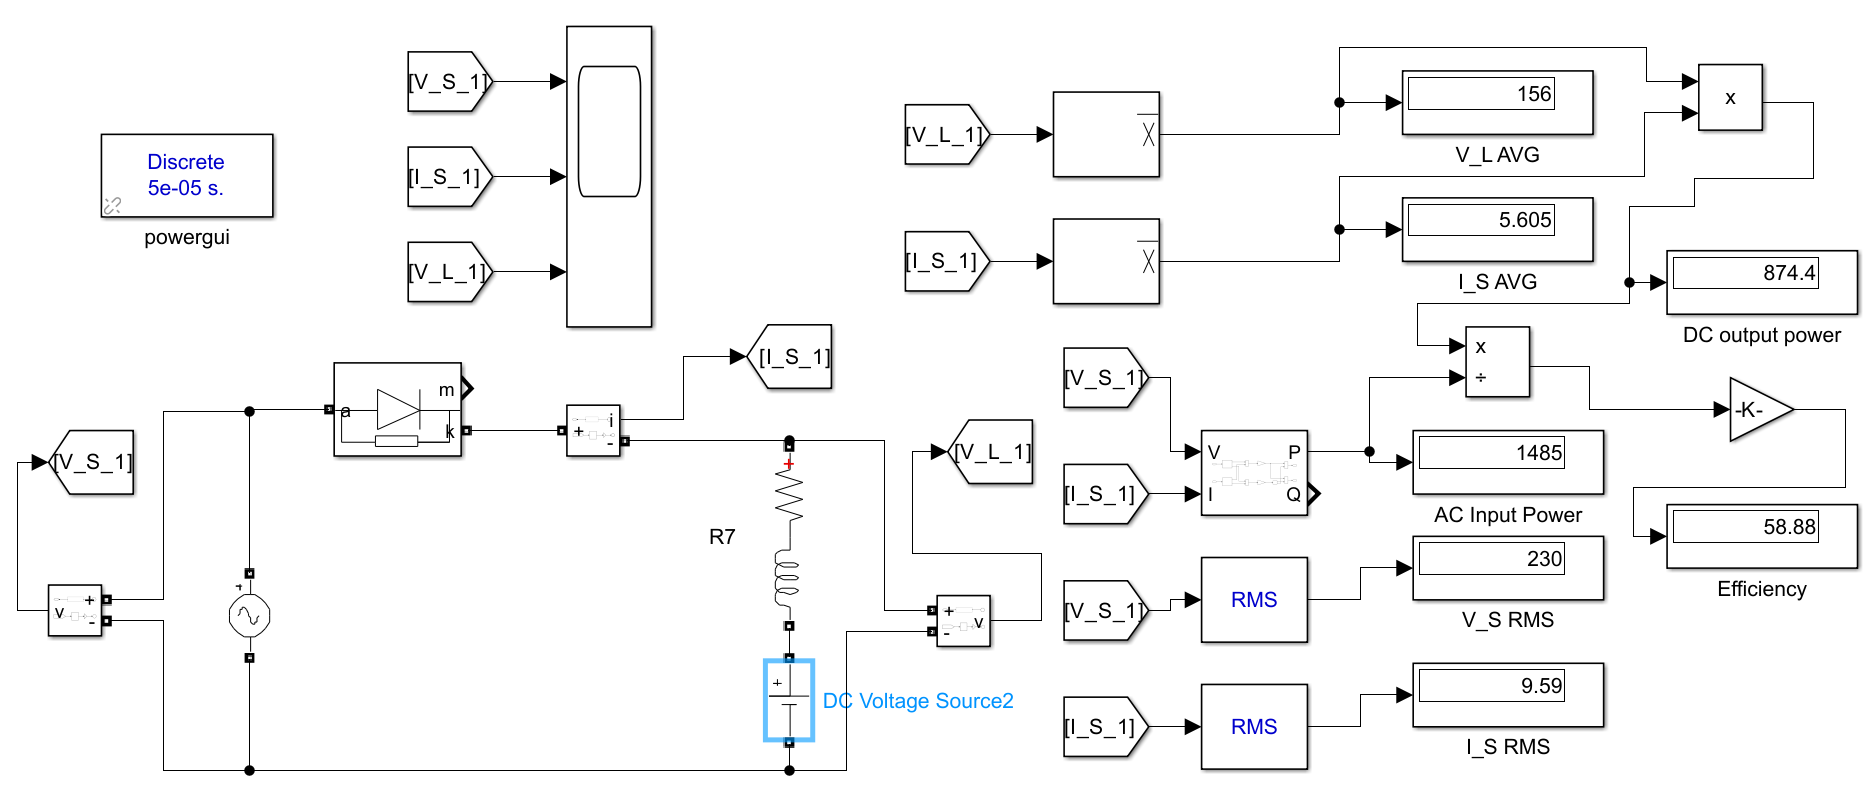
\includegraphics[width=1.0\textwidth]{images/experiment-1/circuit-diagram-experiment-04.png}
    \caption{Circuit for Single Phase Half Wave Uncontrolled Rectifier with RLE load}
    \label{Fig_simulation_circuit_single-phase-half-wave-uncontrolled-rectifier-with-RLE-load}
\end{figure}

\subsection{Components Required}

\begin{table}[h]
    \renewcommand{\arraystretch}{1.3}
    \label{table_components_required_single-phase-half-wave-uncontrolled-rectifier-with-RLE-load}
    \centering
    \begin{tabular}{|c|c|c|c|}
        \hline
        Sr. No & Parameters                     & Ratings            & Quantity \\
        \hline
        \hline
        1      & AC Single Phase Voltage Source & 230V ($ V_{rms} $) & 1        \\
        \hline
        2      & Resistor                       & 10$ \Omega $       & 1        \\
        \hline
        3      & Inductor                       & 10mH               & 1        \\
        \hline
        4      & Diode                          & -                  & 1        \\
        \hline
        5      & DC Source                      & 100V               & 1        \\
        \hline
        6      & Voltmeter                      & -                  & 2        \\
        \hline
        7      & Ammeter                        & -                  & 1        \\
        \hline
    \end{tabular}
    \caption{Components for Single Phase Half Wave Uncontrolled Rectifier with RLE load}
\end{table}




\subsection{Observations}

\begin{table}[h]
    \renewcommand{\arraystretch}{1.3}

    \label{table_observation_single-phase-half-wave-uncontrolled-rectifier-with-RLE-load}
    \centering
    \begin{tabular}{|c|c|c|}
        \hline
        Parameters                              & Theoretical Values & Simulation Values \\
        \hline
        \hline
        AC Input Voltage ($ V_{in,rms} $)       & 230V               & 230V              \\
        \hline
        Output Average Voltage ($ V_{o,avg} $)  & 148V               & 156V            \\
        \hline
        Output Average Current ($ I_{o,avg}  $) & 5.8A               & 5.605A            \\
        \hline
        AC Input Power ($ P_{AC}  $)            & 2389.5 (W)         & 1485 (W)          \\
        \hline
        DC Input Power ($ P_{DC}  $)            & 1071.53 (W)        & 874.4 (W)         \\
        \hline
        Efficiency (\%)                         & 44.84              & 58.88             \\
        \hline
    \end{tabular}
    \caption{Observations for Single Phase Half Wave Uncontrolled Rectifier with RLE load}
\end{table}


The observed simulation results show that the output voltage waveform for the RL load is similar to the input voltage waveform but with a positive DC offset. The rectification process of the circuit converts the negative half cycle of the input waveform into a positive voltage. When the output current falls to zero, the diode stops conducting, and the output voltage becomes a constant 100V, which is equal to the peak value of the input AC voltage.
The efficiency of uncontrolled rectifier with RLE load is 67.88%.

\pagebreak

\subsection{Resultant Waveforms}

% figure that is centered on the page
\begin{figure}[h]
    \centering
    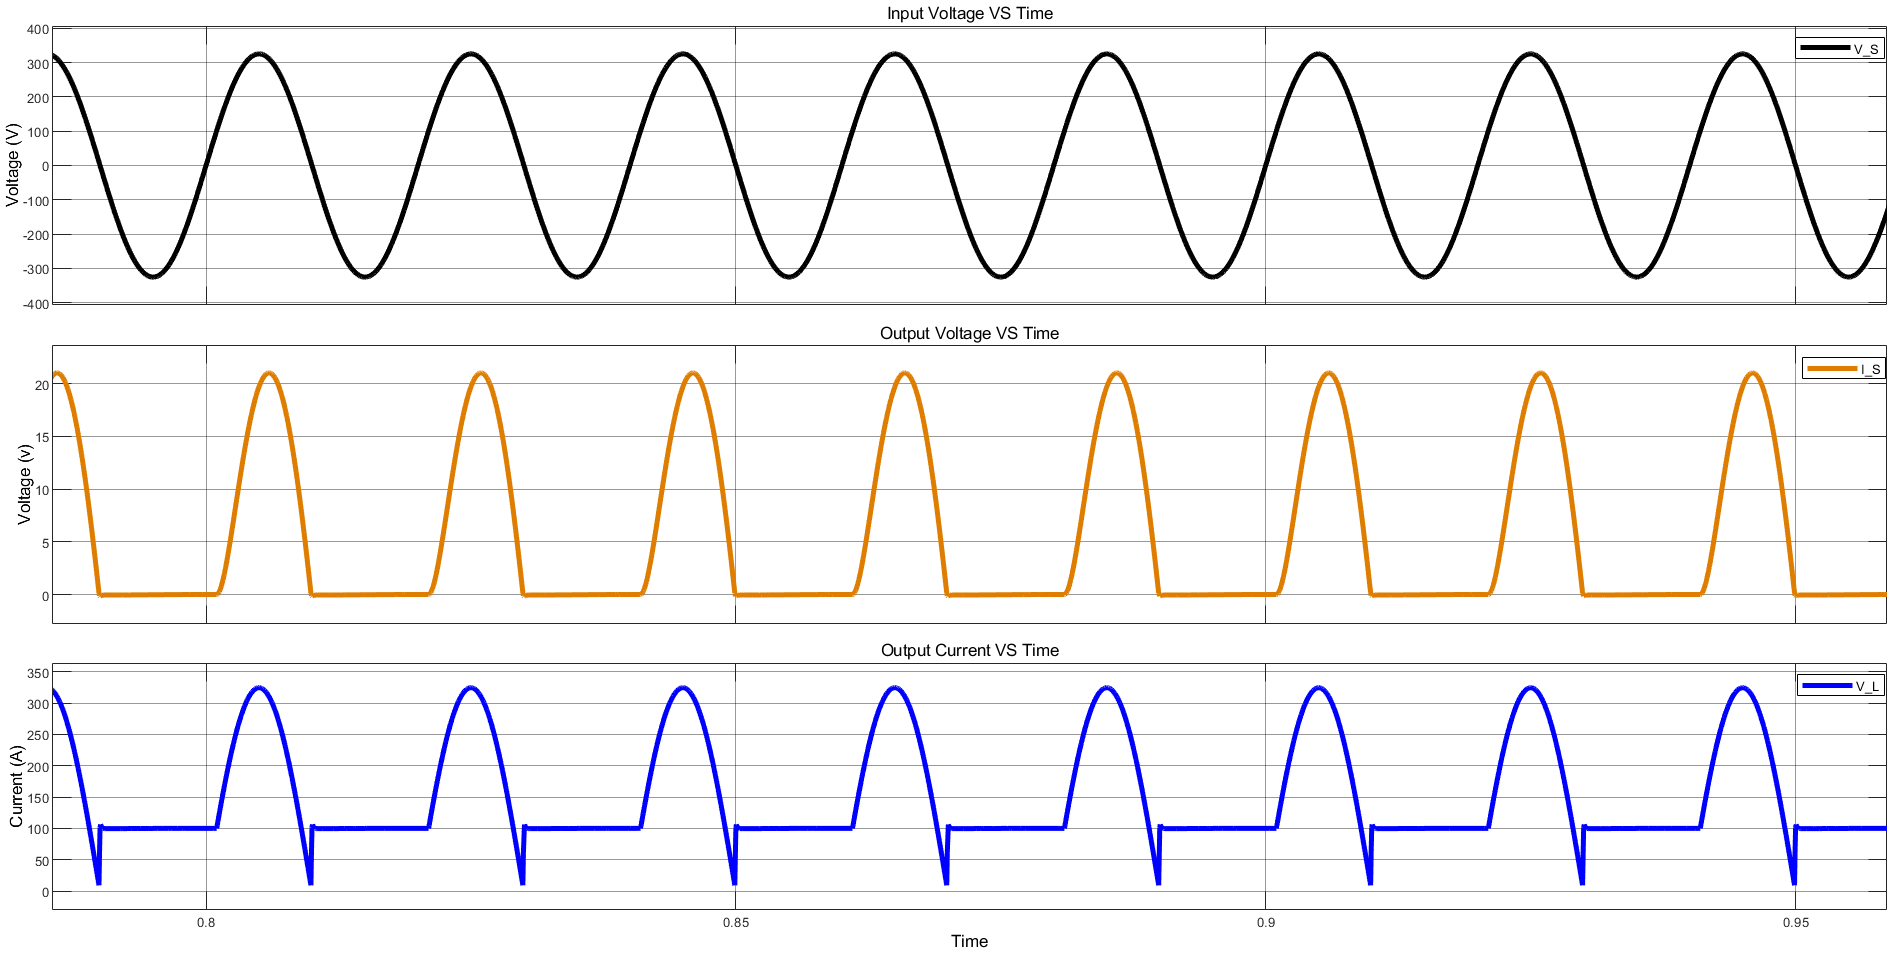
\includegraphics[width=1\textwidth]{images/experiment-1/circuit-scope-experiment-04.png}
    \caption{Scope Waveforms for Single Phase Half Wave Uncontrolled Rectifier with RLE load waveforms}
    \label{Fig_waveform_single-phase-half-wave-uncontrolled-rectifier-with-RLE-load}
\end{figure}

\pagebreak

